\documentclass[tikz,border=12pt]{standalone}
\usepackage[T1]{fontenc}
\usepackage{mathpazo}
\usepackage{amsmath,amssymb}
\usetikzlibrary{arrows.meta, calc}

\definecolor{stblue}{HTML}{7B97AD}
\definecolor{rwgold}{HTML}{B8995E}
\definecolor{sage}{HTML}{7A9A7E}
\definecolor{dkbrown}{HTML}{3D3530}
\definecolor{wmgray}{HTML}{7B7067}
\definecolor{cream}{HTML}{F9F6F0}
\definecolor{border}{HTML}{D4C9B8}
\definecolor{terracotta}{HTML}{C47A6A}
\definecolor{lavender}{HTML}{907EA0}

\begin{document}
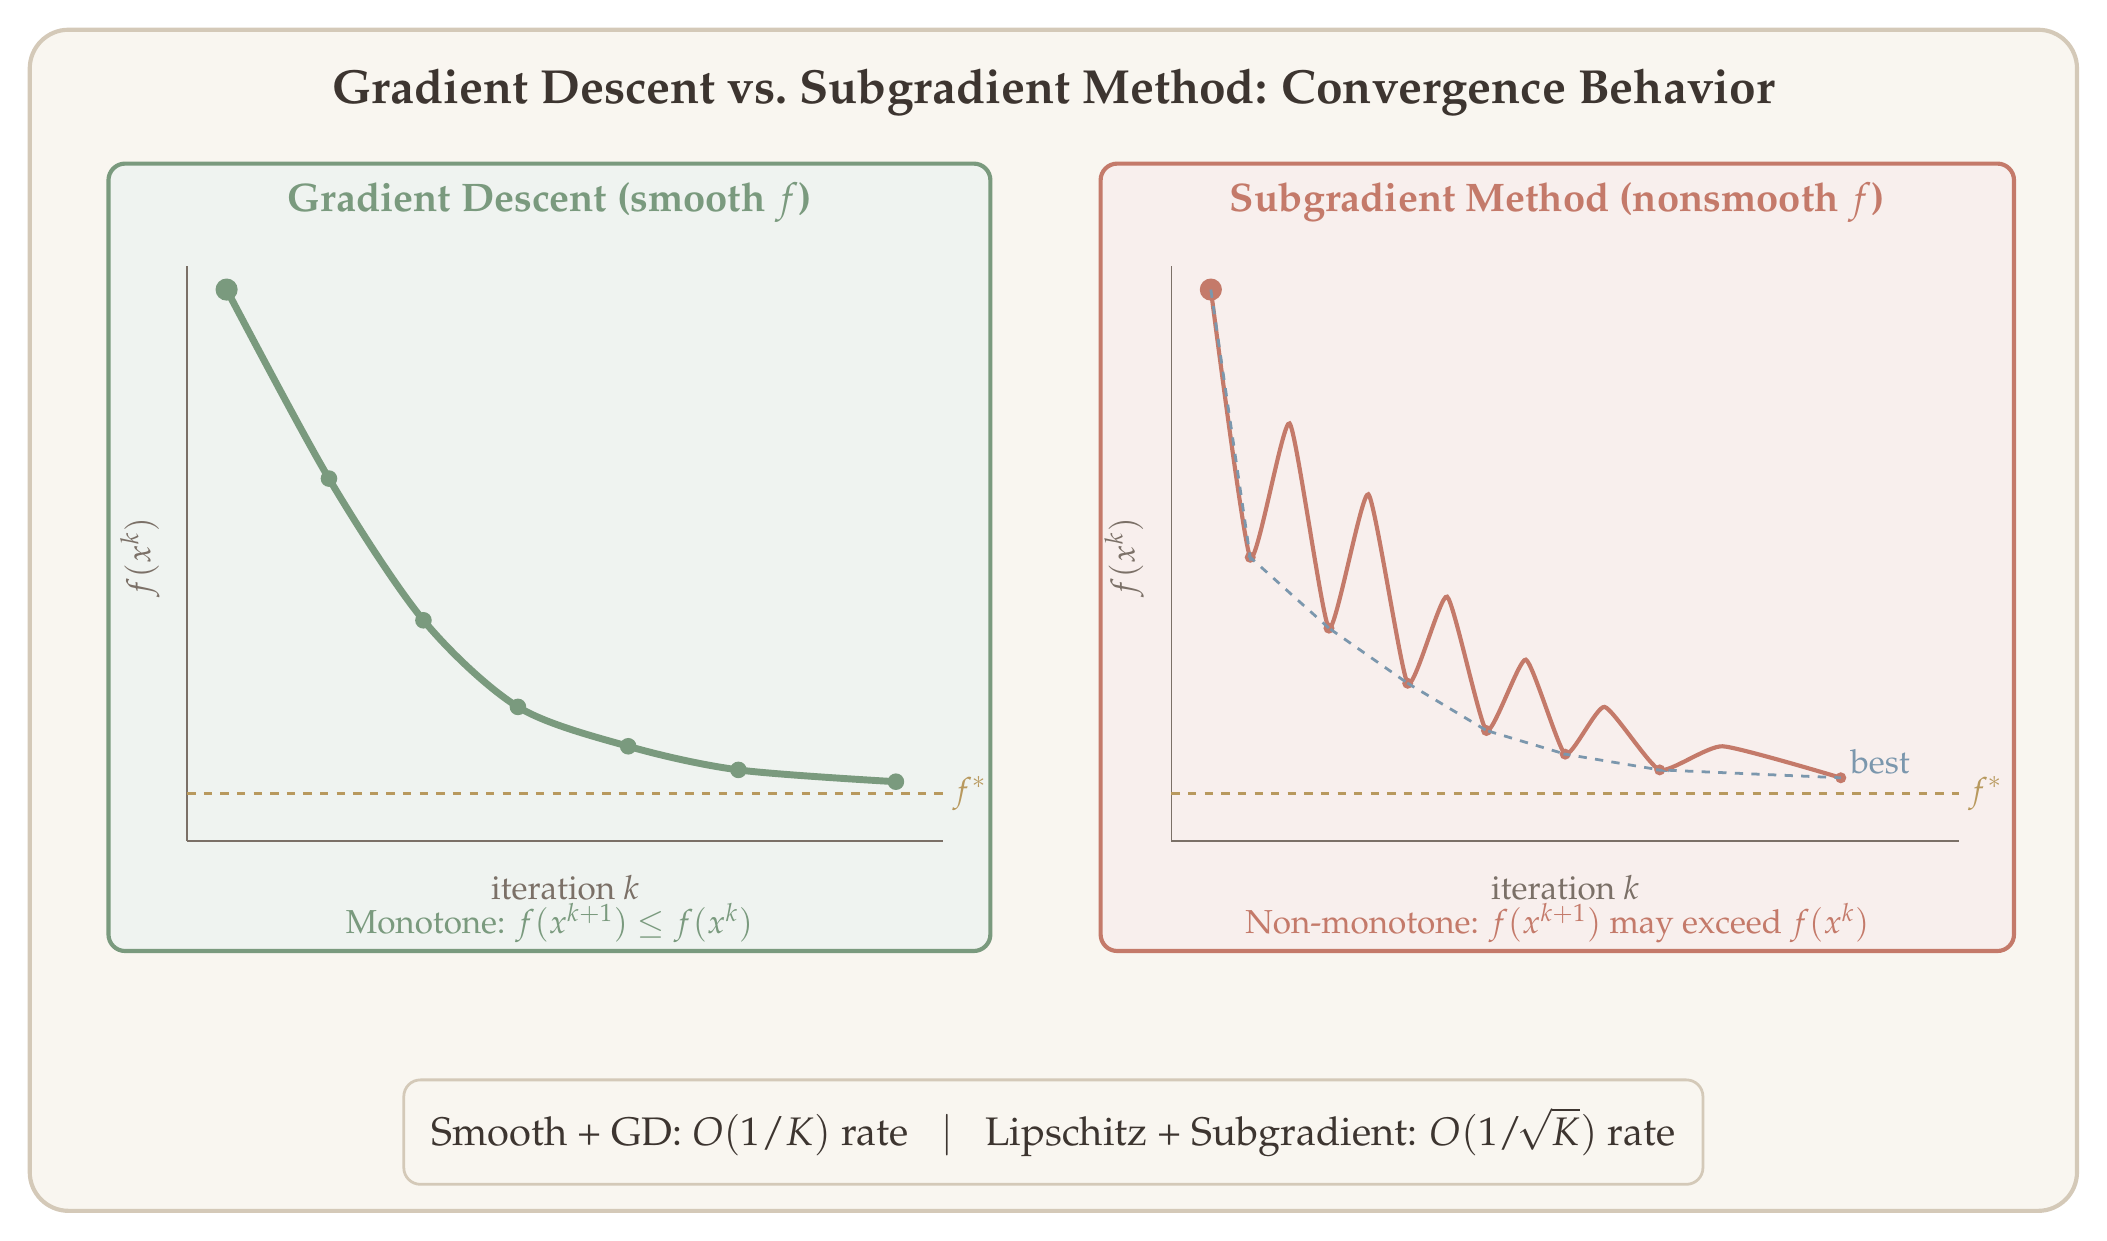
\begin{tikzpicture}[>={Stealth[length=4mm, width=3mm]}]

% Background
\fill[cream, rounded corners=14pt] (-1.0,-2.5) rectangle (25.0,12.5);
\draw[border, line width=1.5pt, rounded corners=14pt] (-1.0,-2.5) rectangle (25.0,12.5);

% Title
\node[text=dkbrown, font=\LARGE\bfseries] at (12.0,11.7)
  {Gradient Descent vs.\ Subgradient Method: Convergence Behavior};

% --- Left panel: GD ---
\fill[sage!12, rounded corners=6pt] (0.0,0.8) rectangle (11.2,10.8);
\draw[sage, line width=1.5pt, rounded corners=6pt] (0.0,0.8) rectangle (11.2,10.8);
\node[text=sage, font=\Large\bfseries] at (5.6,10.3) {Gradient Descent (smooth $f$)};

% Axes
\draw[wmgray, line width=0.6pt] (1.0,2.2) -- (10.6,2.2);
\draw[wmgray, line width=0.6pt] (1.0,2.2) -- (1.0,9.5);
\node[text=wmgray, font=\large] at (5.8,1.6) {iteration $k$};
\node[text=wmgray, font=\large, rotate=90] at (0.4,5.8) {$f(x^k)$};

% f* line
\draw[rwgold, line width=0.8pt, dashed] (1.0,2.8) -- (10.6,2.8);
\node[text=rwgold, font=\large, right] at (10.6,2.8) {$f^*$};

% Monotone decreasing curve
\draw[sage, line width=2.5pt] plot[smooth, tension=0.5]
  coordinates {(1.5,9.2) (2.8,6.8) (4.0,5.0) (5.2,3.9) (6.6,3.4) (8.0,3.1) (10.0,2.95)};
\fill[sage] (1.5,9.2) circle (4pt);
\foreach \x/\y in {2.8/6.8, 4.0/5.0, 5.2/3.9, 6.6/3.4, 8.0/3.1, 10.0/2.95} {
  \fill[sage] (\x,\y) circle (3pt);
}

% Annotation
\node[text=sage, font=\large, align=center] at (5.6,1.15)
  {Monotone: $f(x^{k+1}) \leq f(x^k)$};

% --- Right panel: Subgradient ---
\fill[terracotta!12, rounded corners=6pt] (12.6,0.8) rectangle (24.2,10.8);
\draw[terracotta, line width=1.5pt, rounded corners=6pt] (12.6,0.8) rectangle (24.2,10.8);
\node[text=terracotta, font=\Large\bfseries] at (18.4,10.3)
  {Subgradient Method (nonsmooth $f$)};

% Axes
\draw[wmgray, line width=0.6pt] (13.5,2.2) -- (23.5,2.2);
\draw[wmgray, line width=0.6pt] (13.5,2.2) -- (13.5,9.5);
\node[text=wmgray, font=\large] at (18.5,1.6) {iteration $k$};
\node[text=wmgray, font=\large, rotate=90] at (12.9,5.8) {$f(x^k)$};

% f* line
\draw[rwgold, line width=0.8pt, dashed] (13.5,2.8) -- (23.5,2.8);
\node[text=rwgold, font=\large, right] at (23.5,2.8) {$f^*$};

% Non-monotone oscillating curve
\draw[terracotta, line width=1.5pt] plot[smooth, tension=0.3]
  coordinates {(14.0,9.2) (14.5,5.8) (15.0,7.5) (15.5,4.9)
    (16.0,6.6) (16.5,4.2) (17.0,5.3) (17.5,3.6) (18.0,4.5)
    (18.5,3.3) (19.0,3.9) (19.7,3.1) (20.5,3.4) (22.0,3.0)};
\fill[terracotta] (14.0,9.2) circle (4pt);
\foreach \x/\y in {14.5/5.8, 15.5/4.9, 16.5/4.2, 17.5/3.6, 18.5/3.3, 19.7/3.1, 22.0/3.0} {
  \fill[terracotta] (\x,\y) circle (2pt);
}

% Best iterate line
\draw[stblue, line width=1pt, dashed] plot[smooth, tension=0.2]
  coordinates {(14.0,9.2) (14.5,5.8) (14.5,5.8) (15.5,4.9)
    (15.5,4.9) (16.5,4.2) (16.5,4.2) (17.5,3.6) (17.5,3.6)
    (18.5,3.3) (18.5,3.3) (19.7,3.1) (19.7,3.1) (22.0,3.0)};
\node[text=stblue, font=\large, right] at (22.0,3.2) {best};

% Annotation
\node[text=terracotta, font=\large, align=center] at (18.4,1.15)
  {Non-monotone: $f(x^{k+1})$ may exceed $f(x^k)$};

% Bottom comparison box
\node[text=dkbrown, font=\Large,
      fill=cream, inner sep=10pt,
      draw=border, line width=1pt, rounded corners=6pt]
  at (12.0,-1.5)
  {Smooth + GD: $O(1/K)$ rate $\;\;\vert\;\;$
   Lipschitz + Subgradient: $O(1/\!\sqrt{K})$ rate};

\end{tikzpicture}
\end{document}
